\newpage
\section{Image Classification}\label{ch:image_classification} Image
classification is a difficult problem to solve because images are usually not
ideal. Common issues with images are described in the
following section.

\subsection{Image Variation} One way that images can differ is by
\textit{viewpoint variation}, or when the same object can be oriented in many
ways with respect to the camera. An example of viewpoint variation is shown in
Figure \ref{fig:viewpoint} below:

\begin{figure}[ht!] \centering
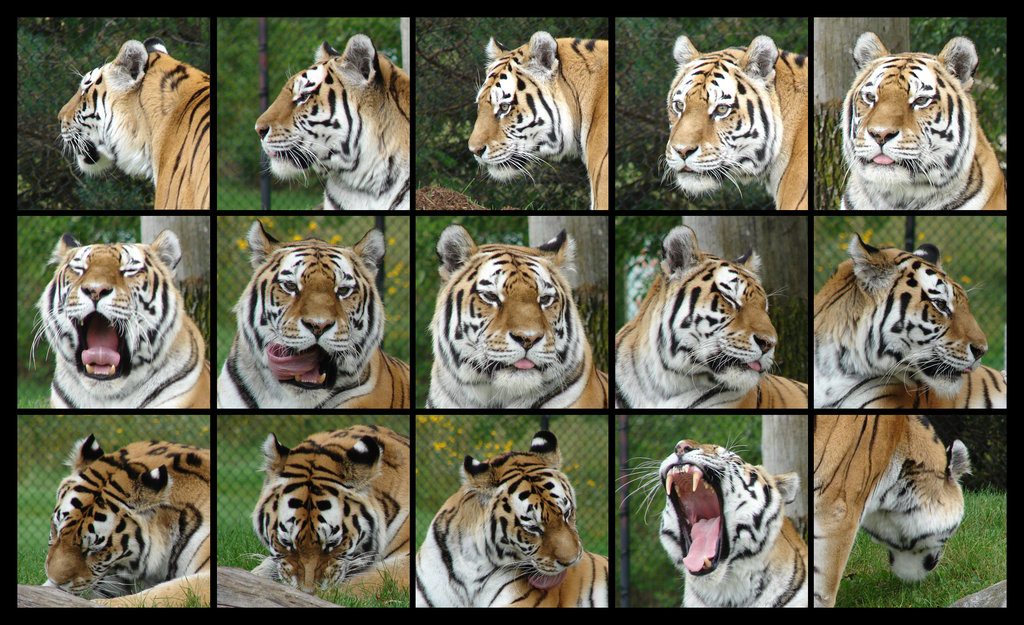
\includegraphics[height=2.5in]{../figures/cat_viewpoint_variation.jpg}
\caption{Tiger's head from many different angles} \label{fig:viewpoint}
\end{figure}

\noindent Above, we see that while each image is very different, our human eye
can detect that we are looking at a tiger. We want an algorithm that can
classify all of these images as a tiger, no matter which direction the image
was taken from.

\noindent Another way in which images can differ is by \textit{scale
variation}, or when there's a difference between sizes of objects within the
same class. Note that this is different than how far away the object is from
the camera when the image is taken; rather, it is more about variation in the
objects themselves.  An example of scale variation is shown in Figure
\ref{fig:scale_variation} below.

% FORMATTING
\newpage

\begin{figure}[ht!] \centering
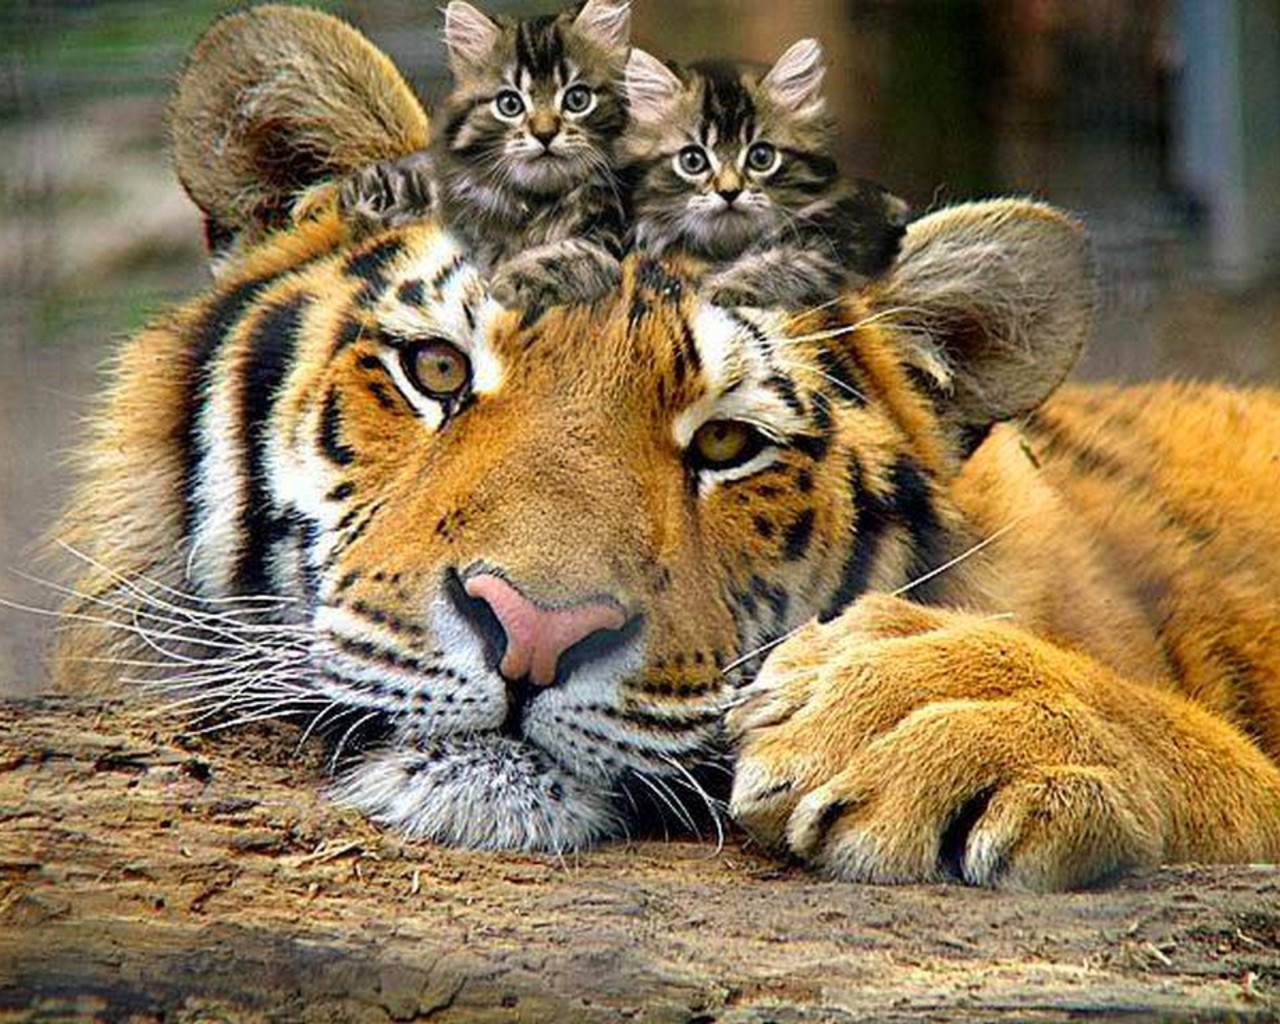
\includegraphics[height=2.5in]{../figures/kitty_scale_variation.jpg}
\caption{Scale variation with cats.} \label{fig:scale_variation} \end{figure}

\noindent We note that, while all of these animals can be classified as cats,
they look quite different. Two of the cats are very small and one of the cats
is significantly larger. This kind of variation occurs regularly within
classes, and it implies that we cannot use the size of an object or its size
relative to other objects as a way to determine its class.

\noindent Objects in an image can also be \textit{deformed}. Since objects of interest
are often not rigid, their shape can vary in many ways. An example of
deformation is shown in Figure \ref{fig:deformation} below.

\begin{figure}[ht!] \centering
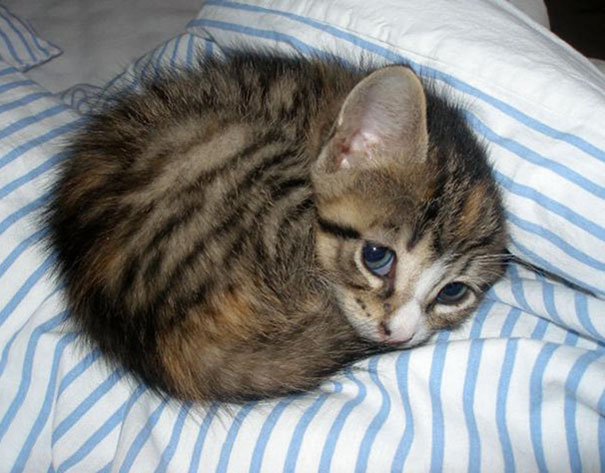
\includegraphics[height=2.5in]{../figures/kitty_deformed.jpg}
\caption{Deformation with cats.} \label{fig:deformation} \end{figure}

\noindent Above, we see that while cats usually have a very specific shape with
protruding legs and tail, this cat is curled up and does not clearly show those
features.

\noindent Sometimes objects in an image can be \textit{occluded}, so only part
of the object is visible. An example of oclusion is shown in Figure
\ref{fig:occlusion} below.

\begin{figure}[ht!] \centering
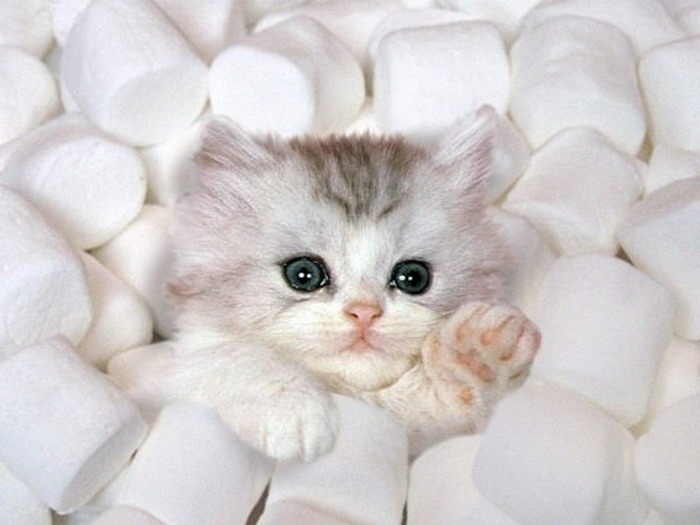
\includegraphics[height=2.5in]{../figures/kitty_occlusion.jpg}
\caption{Occlusion with cats.} \label{fig:occlusion} \end{figure}

\noindent In this image, only the head and two paws of the kitten are visible.
The back two paws, the tail, and most of the kitten's body is hidden, which
makes it harder to classify.

\noindent This image also has another issue known as \textit{background
clutter}. Not only is the cat occluded, but it's surrounded by objects of a
similar color.  From the algorithm's perspective, it can be it difficult to
separate an image's subject from its background.

\noindent Illumination conditions greatly change the pixel values of an image
and sometimes make it difficult to see the object to be classified. An example
of this is shown in Figure \ref{fig:illumination} below.

\begin{figure}[ht!] \centering
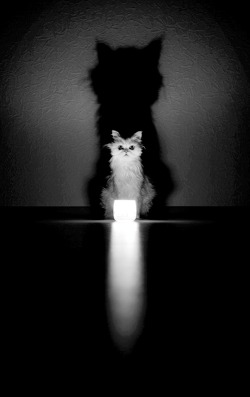
\includegraphics[height=2.5in]{../figures/kitty_illumination.jpg}
\caption{Illumination conditions with cats.} \label{fig:illumination}
\end{figure}

\noindent In this iamge, there's a very stark contrast between the cat and its
background.  Different lighting conditions can also make an object appear more
yellow, more blue, or very dark, which can make it harder to classify.

\noindent Classes of interest can be relatively broad, meaning there's not one
specific way that an object of that class should appear. This issue is
referred to as intra-class variation. An example of this is shown in Figure
\ref{fig:intra_class_variation} below.

\begin{figure}[ht!] \centering
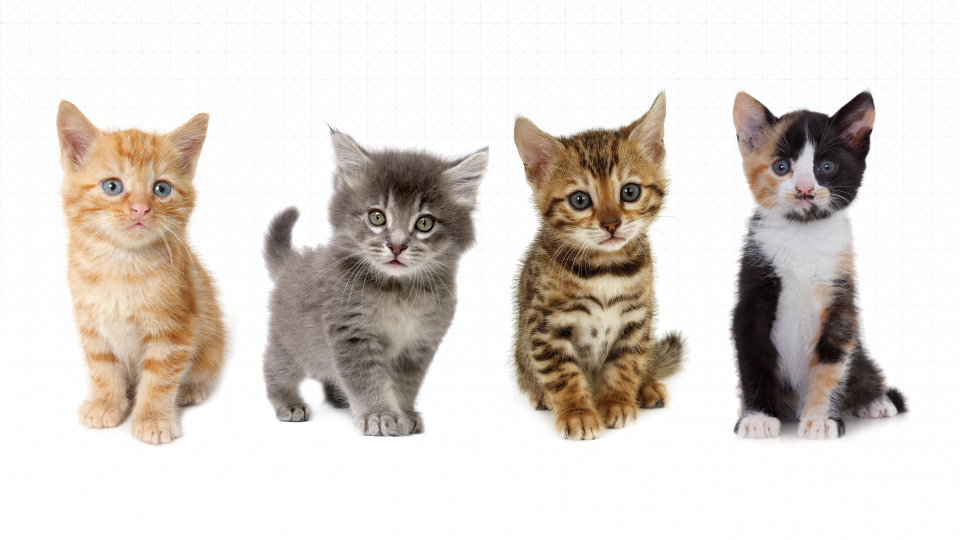
\includegraphics[height=2.5in]{../figures/kitty_intra_class_variation.jpg}
\caption{Intra-class variation with cats.} \label{fig:intra_class_variation}
\end{figure}

\noindent Because there is generally a large amount of variation between
images of the same class as described above, it is not obvious as to how one
would write an algorithm for identifying a specific class within an image.
Instead of specifying what the features for every class might be, we will
instead take a data-driven approach, where we give an algorithm many examples
of each class and allow it to look at those examples and learn what objects of
each class look like, just like a child would do when seeing new objects for
the frist time. This is exactly what neural networks accomplish.

\subsection{Common Datasets for Neural Networks}
To test my implemented network, I looked at two different image classification
datasets; MNIST and CIFAR10. MNIST is a database of images of handwritten
digits 0-9, with the goal being to classify which digit the image represents.
All images in MNIST are $28\times28$ pixels and greyscale.

CIFAR-10 is an object classificaiton dataset. All images in CIFAR-10 are 32x32
pixel images with three color channels: red, green, and blue. This dataset is
generally a more difficult problem to solve than MNIST since the images are
fully colored, meaning there is more data to process, and there's also more
variation between the images in the dataset.
